% IEEE Paper Template for US-LETTER Page Size (V1)
% Sample Conference Paper using IEEE LaTeX style file for US-LETTER pagesize.
% Copyright (C) 2006-2008 Causal Productions Pty Ltd.
% Permission is granted to distribute and revise this file provided that
% this header remains intact.
%
% REVISION HISTORY
% 20080211 changed some space characters in the title-author block
%
\documentclass[10pt,conference,letterpaper]{IEEEtran}
\usepackage{times,amsmath,epsfig}
\usepackage{color}
\newcommand{\res}{CUTE }
%
\title{CUTE: QUery RDF by Table Example}
%
\author{%
% author names are typeset in 11pt, which is the default size in the author block
{First Author{\small $~^{\#1}$}, Second Author{\small $~^{*2}$}, Third Author{\small $~^{\#3}$} }%
% add some space between author names and affils
\vspace{1.6mm}\\
\fontsize{10}{10}\selectfont\itshape
% 20080211 CAUSAL PRODUCTIONS
% separate superscript on following line from affiliation using narrow space
$^{\#}$\,First-Third Department, First-Third University\\
Address Including Country Name\\
\fontsize{9}{9}\selectfont\ttfamily\upshape
%
% 20080211 CAUSAL PRODUCTIONS
% in the following email addresses, separate the superscript from the email address 
% using a narrow space \,
% the reason is that Acrobat Reader has an option to auto-detect urls and email
% addresses, and make them 'hot'.  Without a narrow space, the superscript is included
% in the email address and corrupts it.
% Also, removed ~ from pre-superscript since it does not seem to serve any purpose
$^{1}$\,first.author@first-third.edu\\
$^{3}$\,third.author@first-third.edu%
% add some space between email and affil
\vspace{1.2mm}\\
\fontsize{10}{10}\selectfont\rmfamily\itshape
% 20080211 CAUSAL PRODUCTIONS
% separated superscript on following line from affiliation using narrow space \,
$^{*}$\,Second Company\\
Address Including Country Name\\
\fontsize{9}{9}\selectfont\ttfamily\upshape
% 20080211 CAUSAL PRODUCTIONS
% removed ~ from pre-superscript since it does not seem to serve any purpose
$^{2}$\,second.author@second.com
}
%
\begin{document}
\maketitle
%




\begin{abstract} 
To be filled by Shaoxia.
\end{abstract}

% NOTE keywords are not used for conference papers so do not populate them
% \begin{keywords}
% keyword-1, keyword-2, keyword-3
% \end{keywords}
%
\section{Introduction}
%




\newpage

\null\newpage

\begin{figure*}
\centering
	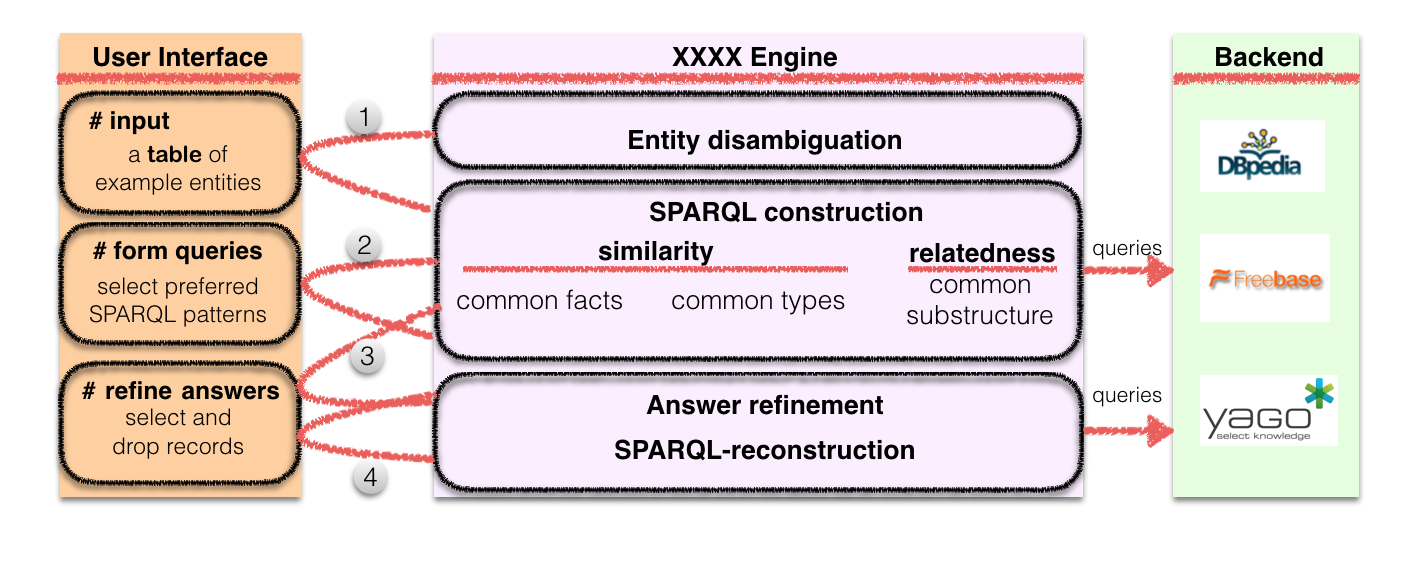
\includegraphics[scale=0.6]{figure/pipeline2}
	\caption{The system architecture (need to be changed  later)}
	\label{pipe}
\end{figure*}

\section{system description}

The design goal of \res is to provide an interface for users to query knowledge graphs more effectively by only providing example results. \res is built on a public SPARQL endpoint\footnote{https://linkeddata1.calcul.u-psud.fr/sparql}. and implemented via Apache Thrift\footnote{https://thrift.apache.org/}. User provides the system with a table of any size containing of some examples she can think of and get all the results she need after interacting with the system. We first formalize our problem, then walk through the system and describe components and implementations in detail.

\subsection{Problem definition}
\textbf{name} takes as input a table, constructs a specific SPARQL query based on the information in the table and returns the results which are a super-set of input entities. The user input may be inaccurate since it's difficult for him/her to know exactly what the entity literals in the graph $G$ look like. \textbf{name} provides a series of candidate entities for users to select.
Formally:

\textup{\textbf{Input:} Assume the user input is a table $\tilde{E}_{m \times n}$ which has $m$ rows and $n$ columns.
Denote the mapping from vague input to accurate entities as $f: \tilde{E}_{m \times n} \rightarrow E_{m \times n}$. For each $\tilde{e}(i,j) \in \tilde{E}_{m \times n}$, $f(\tilde{e}(i,j))=e(i, j)$. $e(i,j) \in  E_{m \times n}$ and $e(i,j) \in G$.}

The $i$-th row  $e(i,0),...,e(i, n-1) $ of $E_{m \times n}$ is a typical result the user desires (i.e., a row in a table that a possible SPARQL query returns).
We assume that entities in the same column
are of the same type and the relations between entities in a row are the same
as that in another row, i.e., the relations between
$e(i, k)$ and $e(i, t)$ are the same as those between $e(j,k)$
and $e(j,t)$.

\textbf{Final output:} A SPARQL query after user selection
$Q$ and the results $R$ after evaluation, $s.t.$ $E_{m \times n} \subseteq R.$ Such queries can be re-constructed iteratively based on user's feedback, as discussed in section...


\subsection{System overview}
Figure \ref{pipe} demonstrates the architecture of \textbf{Name}. 
After receiving user input $\tilde{E}_{m \times n}$, it first maps them to ${E}_{m \times n}$ via entity disambiguation. 
Given the accurate entities we have, it seeks appropriate triple patterns to construct SPARQL queries from two aspects: 1) uncovering similarities among the entities in column $i \ (i = 0,\ldots,n-1)$,
 generating a set of common attributes (including entity types) for each column.
 2) detecting the 
 common relations among entities in a row by constructing one minimal subgraphs for each row and finding the maximal common substructure of these subgraphs.
Our final SPARQL query contains the common structure of the graphs and part of
the common attributes selected by users.

We then display the results returned by a public endpoint to our users and accept their 
feedback of indicating results they tend to drop to reconstruct queries. This can be done iteratively until reaching the 
answers that the user is satisfied with.

\subsection{System components}
We walk through each component of xx and describe design decisions motivated by our observation of our users.

\textbf{[Entity disambiguation]} 
The input of XX can be considered as a table $\tilde{E}_{m \times n}$ (inaccurate user input). We map the input to an accurate entity table $E_{m \times n}$, each element in which is
chosen by the user from the candidate entities we provide, thus
we have all the exact example vertices $V_{input} \subseteq V(G)$ 
in the RDF graph $G$.
We implement this via the JaroWinkler distance algorithm to measure the edit distance between user input strings and entities in the RDF graph. Then, users will be given top $k$ candidate entities based on the distance and choose the one matching her intention to feed into the system. 

\textbf{[Common attributes discovering]}
This module is specific to detect similarities between entities in the same columns. It is composed of two parts: \emph{type inferring} which aims to detect common types of entities and \emph{fact discovering} which 
outputs informative common facts of entities. 
\textbf{Name} infers the common types based on the pre-computed `type' information of the dataset. More specifically,
For entities $(e(1,i),\  e(2,i),..., e(m,i))$ in $E_{m \times n}$ $(i = 1$,...,$n)$,
we consider:
	
\begin{itemize}
    \item the same \emph{types} of $e(j,i),\ j=1,2,...,m$
    \item the same \emph{p} and \emph{o} of triples in which $e(j,i)$
    acts as \emph{s}, $j=1,2,...,m$
    \item the same \emph{s} and \emph{p} of triples in which $e(j,i)$
    acts as \emph{s}, $j=1,2,...,m$
\end{itemize}

\vspace{0.6ex}
In order to speed up the execution, we utilize some pre-stored meta information about the RDF graph (knowledge base) and implement this part via SPARQL queries. Analyzing such information inside the database makes it possible to avoid the shipment of large amounts of data. We then add the user-selected common attributes to the SPARQL queries we are going to construct.

\textbf{[Common relations finding]}
Here we aim to discover relatedness between entities in the same rows. However, not every edge in $G$ has equal contributions in linking related entities. First, for each row $i$ $(i=1,...,m)$, \textbf{Name} constructs a minimal directed graph in terms of edge numbers containing all entities in this row. Among those minimal graphs, it picks up the most `informative' one based on the \emph{Predicate Frequency Inverse Triple Frequency.}\ref{}


%The core idea is Breadth-First-Search. We maintain a queue and two arrays to record the shortest path from some beginning node to a given node  the largest weight under the shortest path.
After building $m$ subgraphs (patterns), \textbf{name} detects the maximal common substructure of these patterns, which can be regarded as the relatedness between input entities. 



\textbf{[Interactively querying]}
Since the maximal common pattern is relatively small in size and contains the necessary semantic information
that we cannot drop any of the triples in the pattern,
we focus mainly on selecting the common attributes
among entities in a column. In a RDF dataset, the attributes of a certain 
entity we detect are always huge in size and some of them may contain less information in constructing SPARQL queries. %For instance, for a certain type of person the user queries, the common attributes `person' is unnecessary in the SPARQL query since it will certainly include some subclass of `person'.
The scope of the concept the common attributes refer to may be neither too general nor too narrow. 
We then ask: \emph{What kind of common attributes meet users' 
expectation of the results most?} This question is difficult to answer given such little information. It's also hard to infer users' real intention only based on a few entities they provide.
For now, we address this problem by interacting with users -- accepting their feedbacks of negative results, reconstructing the SPARQL queries accordingly and returning a new set of answers.
It's often the case that the user searches for an answer for multiple times in a search engine until reaching a satisfying one. It is the same with our system.
The initial SPARQL query outputs a set of tuples that may be answers of interest to the user. Then the user examines the answers, gains some knowledge and picks up some answers against his intention
which will be fed as `negative seeds' into our system to reconstruct the SPARQL queries using the \emph{FILTER NOT EXISTS} and \emph{FILTER} key word. Again, \textbf{name} discovers common attributes (i.e., types and facts) that only belong to negative results and add them to the \emph{`FILTER NOT EXIST'} pattern after user selection.
This process is done iteratively by appending new \emph{`FILTER NOT EXIST'} patterns at the end of the latest SPARQL query after the user feedback.

%We then need to add some triples under `FILETER NOT EXISTS' based on the `negative seeds' users provide. Again, \textbf{name} discovers common attributes of each column of negative and postive entities, which is introduced at \textbf{Common attributes discovering}. The set of negative common attributes subtracts the set of postive ones, and we will get some particular common attributes that only belong to negative results.

\begin{figure*}
    \centering
    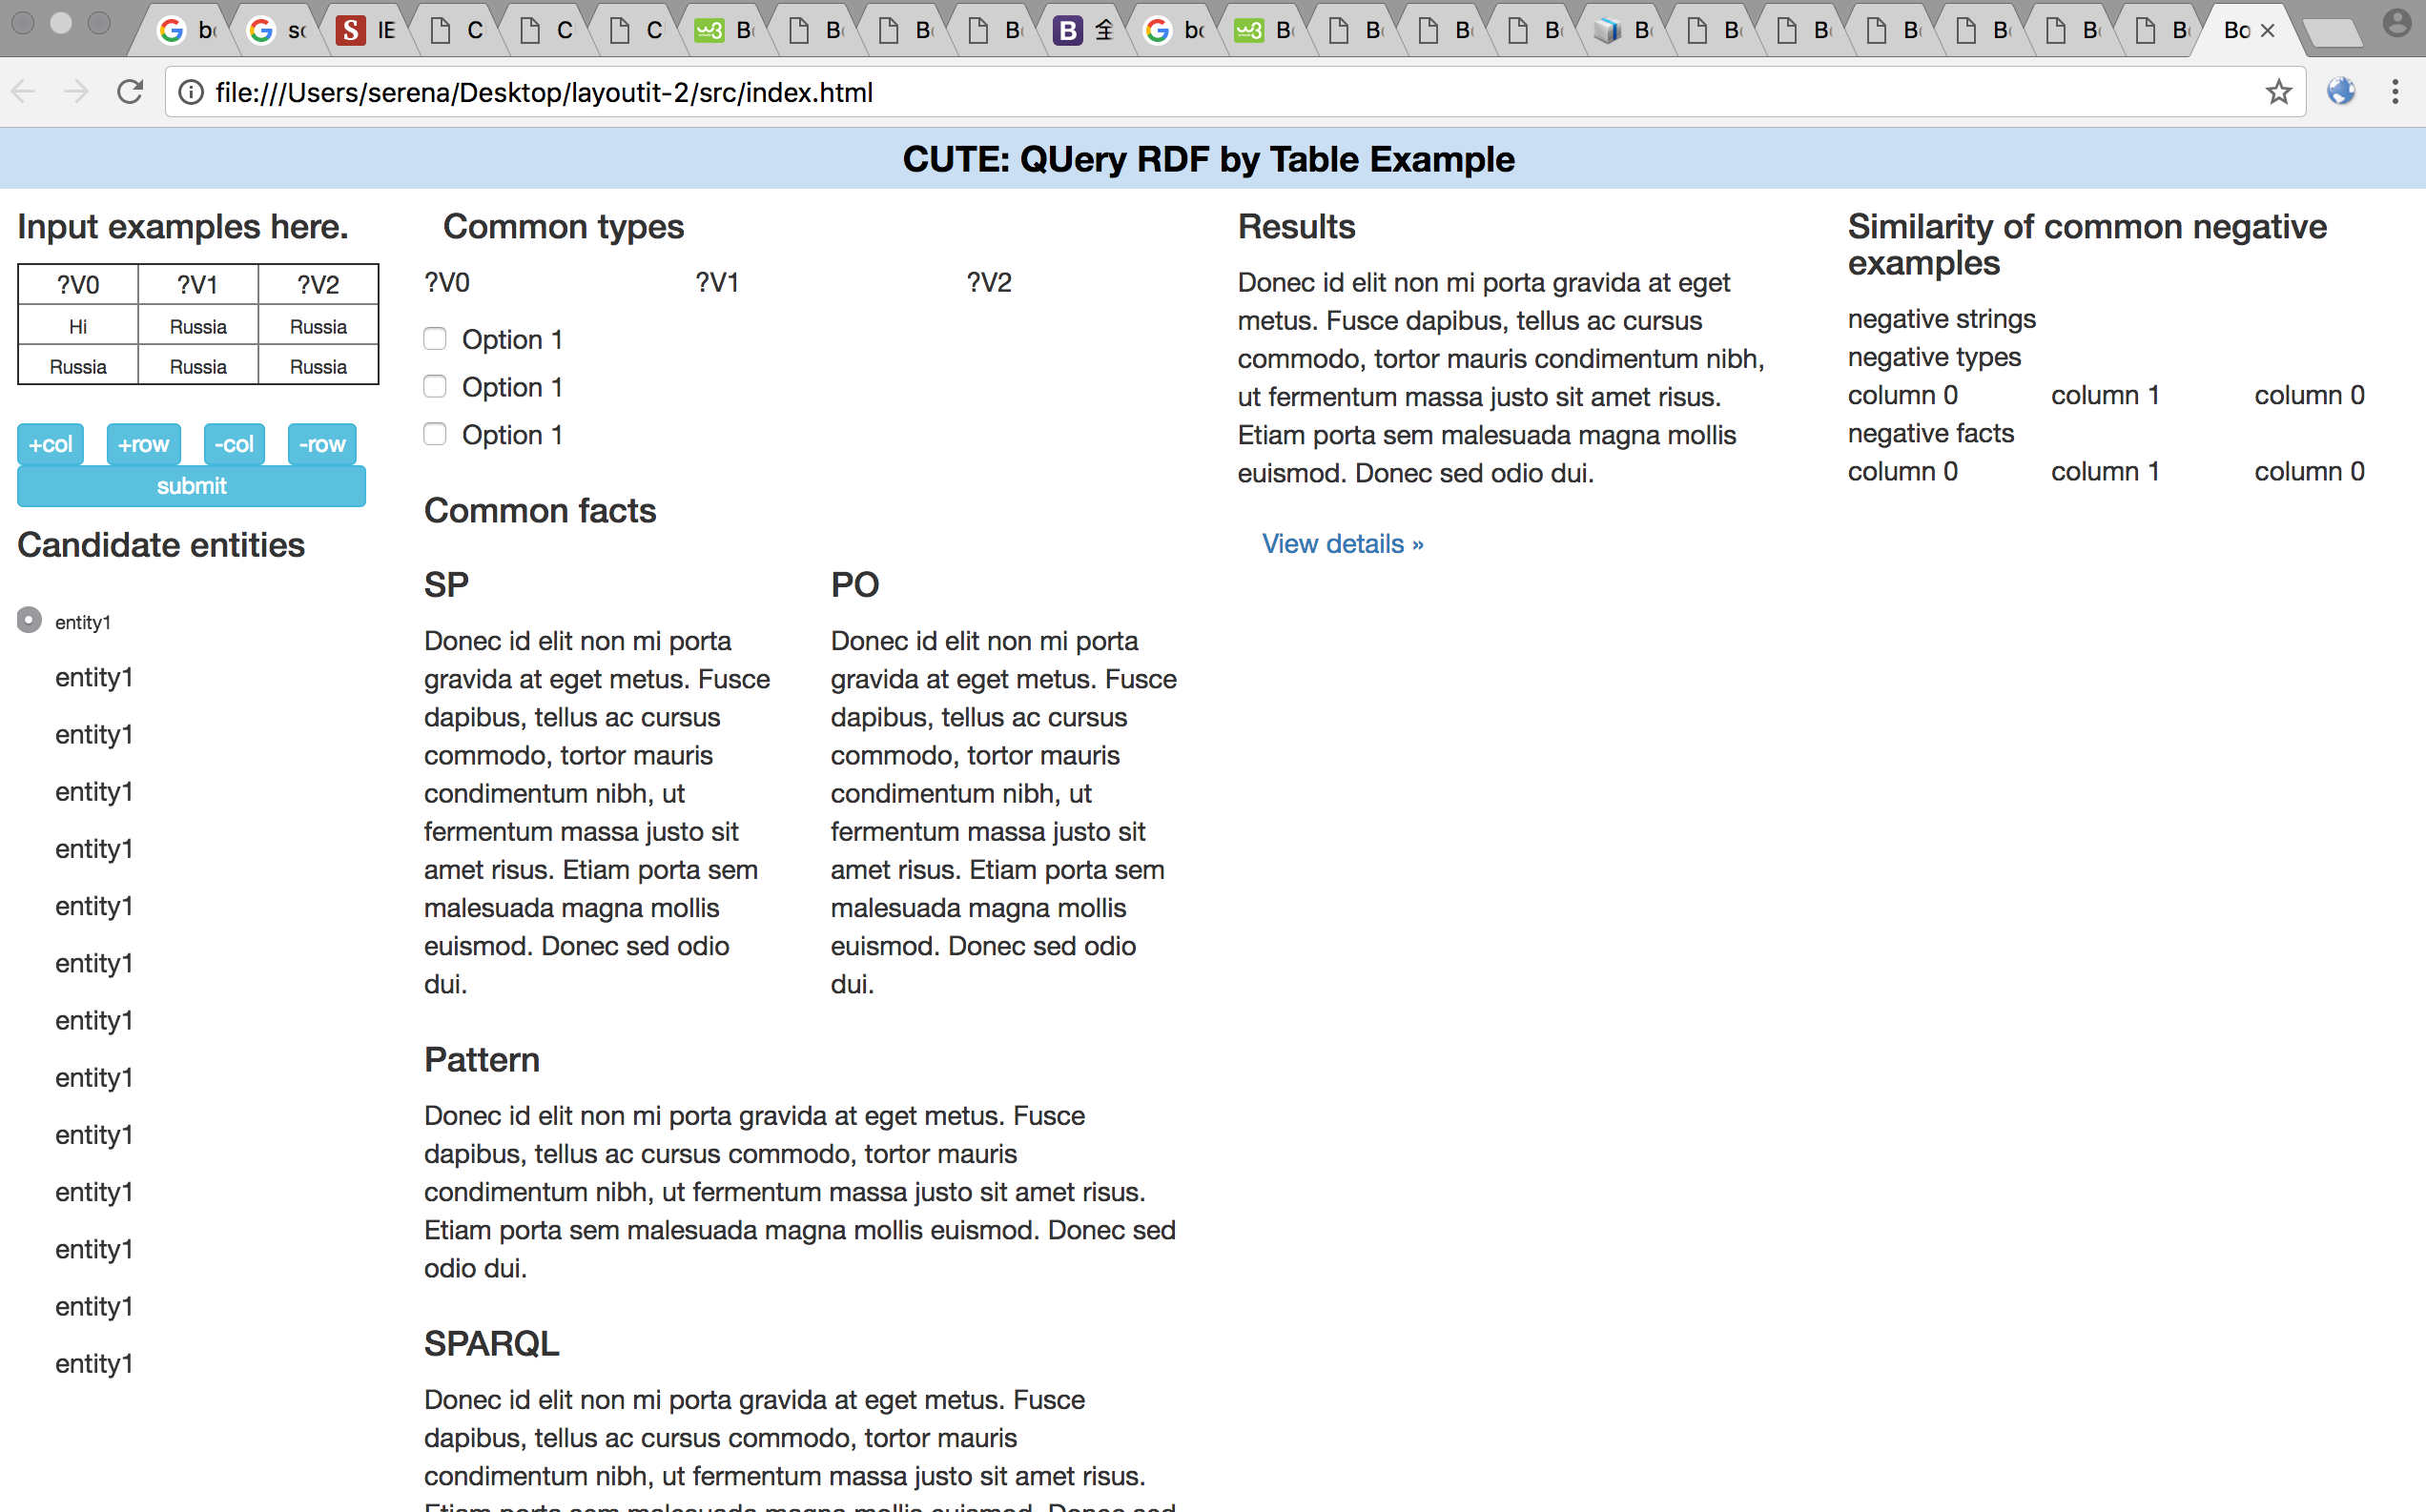
\includegraphics[scale=0.35]{figure/ui_2.png}
    \caption{Should have an interface here.}
    \label{fig:UI}
\end{figure*}


\begin{figure}
    \centering
    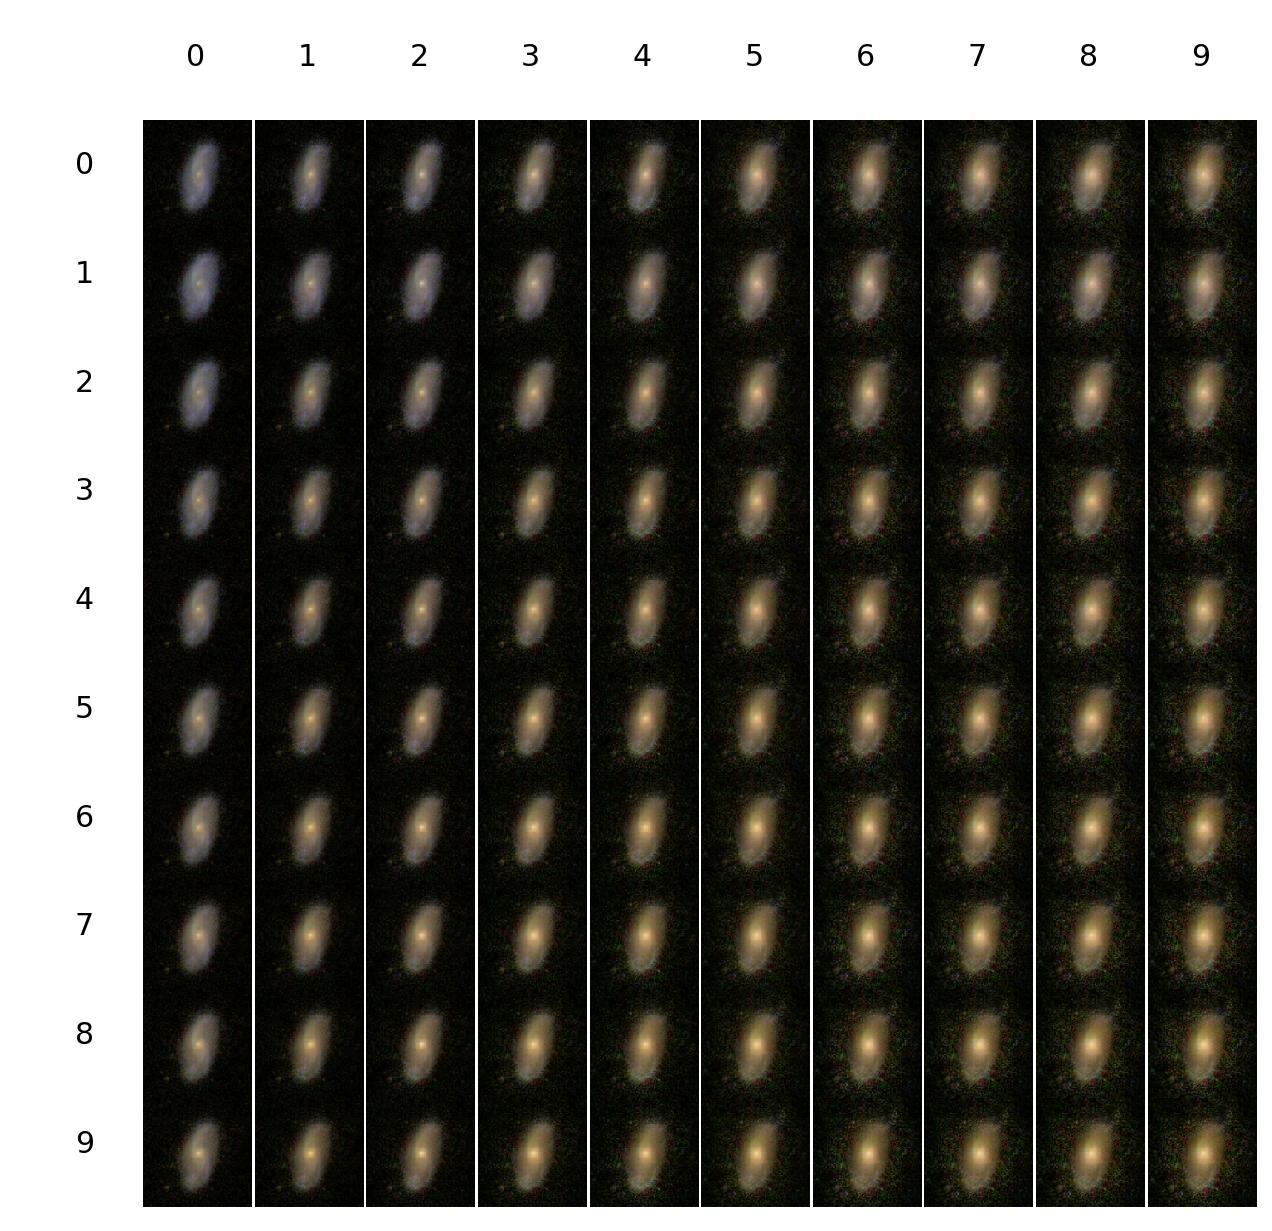
\includegraphics[scale=0.1]{figure/ui.png}
    \caption{Should have a negative example interface here.}
    \label{fig:UI}
\end{figure}

\section{running example}

One of peculiarity of \res is that different from related work, it takes as input entities organized as a general form of tables and can be easily deployed on top of any popular RDF query endpoint.

\textcolor{red}{Notes: add the UI graph later and modify the paragraph below, add something like "As is shown in Figure XX, (q)"}.

We have developed a main running example that will serve as a basis to explain the ideas underlying our framework. Some user might be curious about which celebrities of two generations have acted in the same piece of art work. As is shown in Figure \ref{}, she provides CUTE with two examples: \emph{Dick Van Dyke, Barry Van Dyke, Murder 101} and \emph{Jerry Stiller, Ben Stiller, That's Adequate} because she already knows that \emph{Dick Van Dyke} is the father of \emph{Barry Van Dyke} and they have all acted in \emph{Murder 101}. After the user submits the query in a $2\times3$ table, CUTE will find top-5 candidate entities for each entity. Then the user will select the exact ones to feed into the next component. CUTE will proceed to uncover the similarities between entities in the same column by providing all the common attributes and let the user judge which makes more sense. Here, the user will decide that the entities in the first and second column are all \emph{actors} (of course, they are \emph{living people} and \emph{males}). Meanwhile, CUTE will discover the relatedness between entities and display the pattern to the user. In this case, it discovers that the entities in the first column \emph{hasChild} of the entities in the second column and they all \emph{actedIn} the entities in the third column. The interface shows the corresponding generated SPARQL query for the back-end knowledge graphs (We use Yago as an example here). As we can see, there is no way for our user to exactly write such a complex SPARQL query with the sophisticated literals. At the right side of the interface, CUTE outputs the results of the evaluation of that SPARQL query. The user can refine the answers manually by clicking on the box before any undesired tuples to drop them. The negative examples she provides in this way will be fed into the `Answer refinement' component to reconstruct the query iteratively until she is satisfied.

For instance, in the case where the user would like to know something about the famous scientists and their impactful inventions. She feeds a positive example \emph{Alvin\_Hansen, IS\–LM\_model} into CUTE, and it returns some answers in Figure \ref{?}. After she rejects the entities such as xx and xx, CUTE tries to catch her intention by providing common attributes and common key words of those entities. If she chooses \emph{Other} and \emph{wordnet\_artist\_10982338}, the query will be modified and the answers will be regenerated as shown in xx.

\section{Demonstration Scenario}

For the purpose of the demonstration, we will deploy CUTE on a set of SPARQL endpoints of different linked datasets such as Yago and Freebase. The user will provide some positive examples of her question to inspire CUTE to go through all the components.
During the whole process, the user will interact intensively with CUTE in several ways: selecting the accurate entities from top-k candidate ones, choosing common attributes, and giving feedback. XXXXXXXXXXXXXXXXXXXXXXXXXXXX


\section{Related Work}
(1) \underline{Query reversing engineering.}
\emph{Query reverse engineering} is the general problem of abstracting user examples into an explanatory query. For a query language $L$, a \emph{query-by-example} system is often presented with a database $D$ and $n$-ary relations $S$. The \emph{definability} problem is that whether there exists a query $q$ in $L$ such that $q(D)=S$. 

In the relational database context, this problem is coNEX-
PTIME-complete\cite{barcelo2016complexity}. For SPARQL queries over RDF which is supported by our system, several approaches have been proposed to address this problem in previous work\cite{sparqlbye,querybyexample,reversewww,sapphire}. 
Basically, most of them generate relatively small queries at first and extend the queries by adding interesting patterns. How to choose the patterns, how to rank the results via weighted edges/nodes and how to optimize query evaluation has all more or less been studied.
However, some of the work\cite{reversewww,sparqlbye} focuses on theoretical complexity by assuming that 
the user input is a mapping from variables in SPARQL queries to entities in the knowledge base, which is not of practical use.
\cite{querybyexample} first constructs a weighted subgraph of the knowledge base containing all input entities and then models the answer space as a query lattice to evaluate the queries from bottom to the top.
Although it materializes the results of the queries in the lower layers of the lattice and creates hash tables to speed up the execution, the answer space is still too large to compute efficiently. \cite{discovering} works in the similar way that it evaluates queries as they are extending and does incremental SPARQL pattern matching . But it requires the top-$k$ ranked results must include all input examples. However, it only supports one or two input entities, which is difficult to be used to catch user intent. 

We rely on the public endpoint to do the query optimization and parallelize the whole process to achieve better performance. Also, we impose no constraints on user input and support both positive and negative examples.

(2) \underline{Query relaxation.}
\emph{Query relaxation} is another direction towards solving the usability problem of knowledge graphs. The advantage of \emph{query relaxation} in general is that it can create `cooperative' databases that return answers beyond those specified by a standard query. It has been used successfully in deductive databases\cite{deductive_relax}, relational databases\cite{relational_relax}, XML documents\cite{xml_relax} and knowledge graphs\cite{EKG,sapphire}.
\cite{EKG} first extends the knowledge graph by running open IE, followed by query relaxation techniques such as rewriting predicates, replacing triple patterns and suggesting alternative queries. Similarly, \cite{sapphire} recommends changes of the query to the user based on a predictive user model.
We don't expect our users to input triple-like queries in our system. Instead, they only need to provide several examples, where more users' needs can be satisfied, including whose who have no knowledge about SPARQL. But our system somewhat `relaxes' the query by supporting vague input entities to be mapped into accurate ones later.



\section{Conclusion}
We demonstrate XX, an efficient SPARQL query reversing engineering system which interacts actively with users to obtain accurate results. We show that our system can handle complex query examples with very little human effort and can be deployed as a service on top of any liked datasets. 




\bibliographystyle{IEEEtran}
\bibliography{IEEEabrv,IEEEexample}

\end{document}
